\documentclass[a4paper,12pt]{article} % тип документа
\usepackage[text={180mm, 260mm}, left=15mm, right=15mm]{geometry}
\usepackage{graphicx}
\usepackage{wrapfig}
\usepackage{hyperref}
\usepackage[rgb]{xcolor}	
\usepackage[utf8]{inputenc}	
\usepackage[english,russian]{babel}	
\usepackage{amsmath,amsfonts,amssymb,amsthm,mathtools} 
\usepackage{float} 
\usepackage{wasysym}
\usepackage{fourier} 
\usepackage{array}
\usepackage{soul}
\usepackage{makecell}
\usepackage{fontspec}
\usepackage{indentfirst}
\usepackage{caption}
\usepackage{subcaption}
\setmainfont{NewComputerModern}					
\usepackage{mathtext} 		
\usepackage{pst-node}% http://ctan.org/pkg/pst-node						
\usepackage{multirow}
\hypersetup{colorlinks=true,urlcolor=blue}
\usepackage[rgb]{xcolor}
\usepackage{icomma} 
\usepackage{euscript}
\usepackage{mathrsfs}
\usepackage{enumerate}
\usepackage{graphicx}
\usepackage{booktabs}
\usepackage{cmap}									
\usepackage{tabularx}
\usepackage{tikz}
\usepackage{chngcntr}

\counterwithin*{equation}{section}
\usepackage{longtable}
\title{
	Степанов Линейная алгебра.
	\date{}.
}
\usepackage{easybmat}		
\begin{document}
	\maketitle
	\tableofcontents
	\section{02.02.24 1 лекция}
	\subsection{Ранг Матрицы}
	
	\noindent A $\in$ $M_{m,n}$($\mathbb{R}$).
	Строки столбы матрицы могут быть ЛЗ, ЛНЗ.\\
	
	\noindent $a_1$,$\dotso$,$a_m$ строки ЛЗ $\iff$ $\exists$ $\lambda_1$,$\dotso$,$\lambda_m$ $\in$ $\mathbb{R}$ $ \lambda_1^2 + \dotsb + \lambda_m^2 \neq 0 $ \\
	$\lambda_1 a_1 + \dotsb + \lambda_m a_m = 0 = \overbrace{(0,\dotso,0)}^{m} $\\
	
	\noindent$r_1(A)$ - строчный ранг матрицы A - максимальное количество ЛНЗ строк матрицы A.\\
	0 $\leq$ $r_1(A) \leq m$ \\
	
	\noindent$r_2(A)$ - столбчатый ранг матрицы A - максимальное количество ЛНЗ столбцов матрицы A. 
	0 $\leq$ $r_1(A) \leq n$\\
	\subsection{Минор Матрицы}
	\textbf{Определение 1.} Минором порядка k, где k $1\leq k \leq min\{m,n\}$ называется определителем матрицы,образованной элементами стоящими на пересечение некоторых выбранных k строк и k столбцов матрицы A. \\
	$1 \leq i_1 < i_2 < \dotso < i_k \leq m $\\
	$1 \leq j_1 < j_2 < \dotso < j_k \leq n $\\
	
	$M_{i_1 \dotso i_k}^{j_1 \dotso j_k}$ -- минор, обрзованный строками с номерами $i_1, \dotso, i_k$ и столбцами $j_1,\dotso, j_k$\\
	
	\noindent\textbf{Пример}\\
\[A_{3,4}=
\left(
\begin{BMAT}{cccc}{ccc}
	0 & 2 & 1 & 3 \\
	4 & 5 & 0 & -1 \\
	2 & 2 & 1 & 1 
	\addpath{(0,0,1)rrrrulllld}
	\addpath{(0,2,1)rrrrulllld}
	\addpath{(1,3,1)rdddluuu}
	\addpath{(3,3,1)rdddluuu}
\end{BMAT}
\right)
\]
	$M^4_2 = a_{24} = -1 \quad \quad \quad \quad M_{13}^{24}=\begin{vmatrix}
		2 & 3 \\
		2 & 1
	\end{vmatrix}=-4$\\
	Ранг матрицы A, r(A) = максимальный порядок не нулевого минора матрицы A.
	$r(A) = max\{0 \leq k \leq min\{m,n\}\} | \exists$ ненулевой минор порядка k в A, но миноры большого порядка либо $\nexists$ либо все не равны 0.\\
	\noindent\textbf{Пример}\\
	$	M_{123}^{123}=\begin{pmatrix}
		$0$ & $2$ & $1$\\
		4& $5$ & 0  \\
		$2$ & $2$ & $1$
	\end{pmatrix} \neq 0 \quad \Rightarrow \quad r(A) = 3 $
	\subsection{Теорема об инвариантности ранга при элементарных преобразованиях}
	Если матрица $A'$ получена из матрицы $A$ последовательностью элементарных преобразований строк и столбцов, то $r_1(A')=r_1(A)$ и $r_2(A') = r_2(A)$\\
	\textit{Доказательство после теории размерности векторных пространств}.\\
	
	\textbf{Следствие 1.} 
	$\forall$ матрицы A $r_1(A) = r_2(A)$\\
	\textbf{Доказательство:} Приведем матрицу A к ступенчатому виду   
		\[A'=
		\left(
		\begin{BMAT}{cccccc}{cccccc}
			0 & \dotso & a_{1j_{1}} & \dotso & a_{1j_{n-1}} & a_{1j_{n}}\\
			0 & \dotso & 0 & a_{2j_{2}} & \dotso & a_{2j_{n}} \\
			\vdots &  & \vdots & \vdots & \ddots & \vdots\\
			0 & \dotso & 0 & 0 & 0 & a_{rj_{r}}\\
			0 & \dotso & 0 & 0 & 0 & 0\\
			0 & \dotso & 0 & 0 & 0 & 0
			\addpath{(2,6,1)drdrdrdr}
		\end{BMAT}
		\right) \quad 1 \leq j_1 < j_2 < \dotso < j_r \leq n \qquad a_{1j_1},\dotso ,a_{rj_r} \neq 0\] 
	  Далее поделим k-ую строку на $a_{kj_k}$ и переместим столбы $j_1, \dotso, j_r$ в начало матрицы.
	  
	  $$
	  A' \Rightarrow A'' = \left(
	  \begin{BMAT}{cccc}{cccc}
	  	1 & a_{12}'' & \dotso & a_{1n}''\\
	  	0 & 1 & a_{23}'' & \dotso \\
	  	\vdots & \vdots & \ddots & \\
	  	0 & 0 & \dotso & 1\\
	  	%\addpath{(2,6,1)drdrdrdr}
	  \end{BMAT}
	  \right)
	  $$
	  Из второго столбца вычтем первый с коэффициентом $a_{12}'' \dotso$  из n-го 1-й с коэффициентом $a_{1n}''$ и т.д для 2-го столбца и 2 строки и т.д. 
	  \[
	  A\sim A''' = 
	  \left( \begin{array}{c|c}
	  	E_r & 0 \\
	  	\midrule
	  	0 & 0 \\
	  \end{array}\right)
	  \]
	  $из Teop_1 \Rightarrow r_i(A) = r_i(A'''), i = 1,2$\\
	  Первые $r$ строк матрицы $A'''$:\\
	  $e_1 = (1,0,\dotso,0, \dotso,0)$\\
	  $e_2 = (0,1,\dotso, 0, \dotso,0)$\\
	  $ \qquad \vdots $\\
	  $e_r = (0,0,\dotso,1,\dotso,0)$\\ 
	  
	  Если $\Sigma \lambda_i e_i = 0 = (0,\dotso, 0) \Rightarrow (\lambda_1, \dotso, \lambda_r, \dotso,0) \Rightarrow \lambda_1 = \dotsb = \lambda_r = 0 \Rightarrow $ Эти строки ЛНЗ $\Rightarrow r_1(A''') = r$.\\
	   Аналогично $r_2(A''') = r \Rightarrow r_1(A) = r_2(A)$ Ч.Т.Д.\\
	   
	   \textbf{Замечание}  
	   Вычисление ранга матрицы методом элементарных преобразований: Нужно привести матрицу А к ступенчатому виду путём преобразований строк.
	   Тогда $r_1(A) = r_2(A) = r$ -- количеству ненулевых строк в ступенчатом виде.\\
	   
	   \textbf{Определение 2.} Пусть M -- некоторый минор матрицы A минор $M'$ матрицы А называется окаймляющим для М если $M'$ получается из М добавлением одной строки и одного столбца.\\
	   Пример:
	   $$
	   A=\begin{pmatrix}
	   	1 & 2 & 3 & 4 \\
	   	0 & 0 & 1 & 1 \\
	   	2 & -1 & 3 & 2
	   \end{pmatrix} \quad M=M_{13}^{13}=\begin{vmatrix}
	   1 & 3 \\
	   2 & 3
	   \end{vmatrix}=-3
	   $$
	   Окаймляющие: $M'^{123}_{123}, \ M'^{134}_{123}$\\
	   
	   \textbf{Определение 3} 
	   Минор M матрицы А называется базисным если M $\neq$ 0, а все его окаймляющие миноры либо $\nexists$, либо равны 0. Строки и столбцы входящие в базисные миноры называются базисными.\\
	   
	   \subsection{Теорема о базисном миноре}
		Базисные строки (столбцы) любой матрицы ЛНЗ. Остальные строки(столбцы) линейно выражаются через  базисные.\\
		\textbf{Доказательство:} Для строк, для столбцов аналогично.
		Если базисные строки ЛЗ, то и строки базисного минора ЛЗ $\Rightarrow$ он равен 0 -- противоречие.\\
		Будем считать, что базисный	 минор М = $M_{1,\dotso,r}^{1,\dotso,r}$
		Рассмотрим определители $M'$, которые получаются добавлением к M i-й строки,  i > r и $\forall$ столбцов матрицы А.\\
		Если мы добавим j-й столбце с $j \leq r$ то в  $M'$два одинаковых столбца $\Rightarrow M' = 0$.\\
		Если $j > r$, то $M'$ -- окаймлённный минор для М $\Rightarrow M' = 0$
		$$
		0 = M' =\begin{vmatrix}
			a_{11} & \dotso & a_{1r} & a_{1j} \\
			\vdots & \ddots &\vdots & \vdots\\
			a_{r1} & \dotso & a_{rr} & a_{rj}\\
			a_{i1} & \dotso & a_{ir} & a_{ij}
		\end{vmatrix} = \text{(Разложим по последнему столбцу)}=A'_{1j}a_1j
 + A'_{2j}a{2j} + \dotsb + A'_{rj}{rj}+Ma_{ij} = 0	  $$
 \begin{equation}
 	\label{1}
 	a_{ij} = -\dfrac{A_{1j}'}{M}a_{1j} - \dotso - \dfrac{A_{rj}'}{M}a_{rj} \quad \forall j = 1,\dotso ,n
 \end{equation}
 Формула \eqref{1} выражает элемент i - й строки через соответствующие элементы 1-й, ... , r-й строк. Коэффициенты не зависят от j $\Rightarrow$ i-я строка линейно выражается через базисные строки. ЧТД.\\
 
 
 \textbf{Следствие 2(Теорема о ранге матрицы)} 
$\forall$ матриц А $r_1(A) = r_2(A) = r(A)$ и равны порядку любого базисного минора. 

\textbf{Доказательство}
$r_1(A) = r_2(A)$ -- уже доказано. Пусть M -- базисный минор матрицы A. $M_{12\dotso r}^{12\dotso r}$. (r+1)--я,$\dotso$,m--я строки -- линейная комбинация базисных строк.
$$
A\sim\begin{pmatrix}
	a_{11} &  a_{12} & \dotso & a_{1n} \\
	\vdots & \vdots &\ddots & \vdots\\
	a_{r1} & a_{r2}& \dotso & a_{rn}\\
	0 & 0 &\dotso & 0\\
	0 & 0 &\dotso & 0
\end{pmatrix} = A' \quad \text{из теоремы 1} \Rightarrow r_1(A) = r_1(A')
$$
Строки (1),$\dotso$,(r) ЛНЗ $\Rightarrow r_1(A') = r$. $r$ -- порядок базисного минора. Если $M$ -- максимальный по порядку минор $\neq$ 0, то он автоматически базисный $\Rightarrow r(A) = r = r_1(A) = r_2(A)$

\textbf{Определение 4}
Рангом матрицы А называется число rkA определённое любым выше указанным эквивалентным способом.
\section{09.02.24 2 лекция}
\subsection{Определение 1. Векторное(линейное) пространство}
	\indent Векторное(Линейное) пространство -- это множество $V$ с введенными на нём двух операций + и $\lambda \cdot \ , \lambda \in \mathbb{R}$ которые удовлетворяют следующим условиям( аксиомам векторного пространства)
	\begin{enumerate}
		\item $\forall x,y,z \in V \ (x+y) +z = x+(y+z) \ \text{-- ассоциативность}$
		\item $\forall x,y \in V \ x+y = y+x \ \text{-- коммутативность}$
		\item $ \exists 0 \ \text{--нулевой вектор}: \forall x \in V \ x+0 = x $
		\item $\forall x \in V \ \exists -x \in V : \ x+(-x) = -x+x = 0$\\
		(V,+) -- образуют Абелеву группу.
		\item $\forall \lambda \in \mathbb{R} \ \forall x,y \in V \ \ \lambda (x+y) = \lambda x + \lambda y$
		\item $\forall \lambda, \mu \in \mathbb{R} \ \ \forall x \in V  \ \ ( \lambda + \mu )x = \lambda x + \mu x $
		\item $\forall \lambda,\mu \in \mathbb{R} \ \ \forall x \in V \ \  \lambda(\mu x) = (\lambda \mu) x$
		\item $\forall x \in V \ \ 1\cdot x = x$
	\end{enumerate}
	
	\textbf{\fbox{Замечание}}\\
	\indent Аксиома 2 следует из остальных, докажем это\\
	\begin{equation}
	 (1+1)(x+y) \stackrel{5}{=} (1+1)x + (1+1)y \stackrel{6,1}{=} 1\cdot x + 1\cdot x + 1 \cdot y + 1 \cdot y \stackrel{8}{=} x + x + y + y
	\end{equation}
	\begin{equation}
	 (1+1)(x+y) \stackrel{6}{=} 1\cdot(x+y) + 1(x+y) \stackrel{5, 1}{=} 1\cdot x + 1 \cdot y + 1 \cdot x + 1 \cdot y \stackrel{8}{=} x + y + x + y
	\end{equation}
	(1) и (2) равны $\Rightarrow x+x+y+y = x+y+x+y$. Из 4 аксиомы $\exists -x, -y $ прибавим их слева и справа $\Rightarrow 0+x+y+0 = 0+y+x+0 \stackrel{3}{\Rightarrow} x + y = y+x$\\
	
	\textbf{\fbox{Простые следствия из аксиом}}\\
	\begin{enumerate}
		\item $0 \in V \ \text{единственный: если $0'$ -- второй нулевой вектор. то } 0 + 0' \Rightarrow 0' = 0$
		\item $\forall x \in V \ \ -x \text{ тоже единственный: пусть $-x'$ -- второй } \\-x + x + (-x') = -x' + 0 = -x' \\ -x + (x+(-x')) = -x + 0 = -x \Rightarrow -x' = -x$
		\item $\forall x \in V \  0 \cdot x = 0 : \quad (0+0)x \stackrel{0+0 = 0}{=} 0 \cdot x = 0\cdot x + 0\cdot x \Rightarrow \text{добавим противоположный вектор} \ 0 \cdot x \Rightarrow 0 \cdot x = 0$
		\item $\forall \lambda \in \mathbb{R}\ \  \lambda \cdot 0 = 0 \text{ рассмотрим } \lambda \cdot (0+0) \text{ доказательство аналогично 3) }$
		\item $\forall x \in V \ -x = (-1)x: \text{ Рассмотрим выражения }(1-1)\cdot x \\ 0\cdot x = 0 \text{ из (3) с другой стороны: } (1-1)\cdot x = 1\cdot x + (-1)x = x+(-1)x \ \Rightarrow \ x + (-1)x = 0 \ \Rightarrow \text{из единственности противоположного вектора} (-1)x = -x$
	\end{enumerate}
	
	Определим операцию вычитания векторов: $x- y \stackrel{def}{=} x+(-y)$\\
	
	\textbf{\fbox{Примеры}}\\ 
	\begin{enumerate}
	\item[0.] ($V_3$, x ,$\lambda \cdot$)
	\item[1.] {0} -- векторное(линейное) пространство из 1 элемента (нулевое векторное пространство) 
	\item[2.] $\mathbb{R}$ с обычными операциями 
	\item[3.] пусть $I$ -- некоторое множество, $(V_i)_{i \in I}$ -- семейство векторных пространств
	\end{enumerate}
	
	\subsection{Определение 2. Прямое произведение}
	\indent Прямым произведением семейства $(V_i)_{i \in I}$ называется множество\\ $\underset{i \in I}{\prod} V_{i} = \{x: I \to \underset{i \in I}{\bigcup} V_i | \ \forall i \in I \ \ x_i \in V_i \}$ с операциями $(x+y)(i)  \stackrel{def}{=} x(i) + y(i)$ -- сумма в $V_i$ и \\$(\lambda x)(i) = \lambda x(i)$ -- умножение на скаляр в $V_i$\\
	$\prod V_{i}, +, \lambda \cdot$ -- векторное пространство\\
	
	Например, докажем что аксиома 5 справедлива в $V_i$.\\
	 $(\lambda \cdot (x + y))(i) = \lambda[(x+y)(i)] = \lambda(x(i) + y(i)) = \lambda\cdot x(i) + \lambda \cdot y(i) = (\lambda x)(i) + (\lambda y)(i) = (\lambda x + \lambda y) (i) \Rightarrow \lambda(x+y) = \lambda x + \lambda y$ Ч.Т.Д.\\
	 
	 Также докажем что аксиома 3 справедлива для $V_i$:\\
	 0 в ${\prod} V_{i}$ -- это функция которая $\forall i \in I \ 0(i) = 0 \ \in V_i$\\
	 
	 \textbf{\fbox{Важные частные случаи}}\\ 
	 \begin{enumerate}[a.]
	 	\item Пусть все $ \ V_i \in \mathbb{R}$: Тогда $\underset{i \in I}{\bigcup} V_i = \mathbb{R}$\\
	 	$\prod V_i$ -- это множество всех функций из I в $\mathbb{R}$ с обычными операциями.\\
	 	Обозначим : $\prod V_i = R^I = \{f: I \to \ \mathbb{R} \}$\\
	 	$A = \{a_1, \dots, a_m \} \quad B = \{b_1, \dots, b_n\}$ всего имеем $n^m$ отображений из A в B
	 	\item $I = \{1,2, \dots, n\},\ V_i = \mathbb{R} \ \forall i$\\
	 	Обозначение $R^i = R^n = \{(x_1, \dots, x_n)| x_1, \dotso, x_n \ \in \mathbb{R}\}$\\
	 	$x+y = (x_1 + y_1, \dotso, x_n + y_n)$;   $\lambda\cdot x = (\lambda x_1, \cdots, \lambda x_n)$\\
	 	$R^n$ -- n-мерное арифметическое пространство 
	 	\item $I = \{1,2\}$, $V_1 = U$, $V_2 = W$ -- два разных пространства\\
 	 	$\underset{i \in I}{\prod} V_i = U\times W$ -- прямое произведение\\
 	 	$U \times W = \{ (u,w) u \in U; w \in W\}$\\
 	 	$(u,w) + (u',w') = (u + u', w + w')$ -- в такой ситуации $U \times W$ называется прямой суммой  $U$ и $W$ и обозначается $\oplus $\\
 	 	$\lambda(u,m) = (\lambda u + \lambda w)$\\
 	 	\end{enumerate}
 	 	\subsection{Определение 3. Подпространство}
 	 	
 	 	V -- векторное пространство. Подмножество $U \subseteq V$ называется векторным(линейным) подпространством если выполнены следующие условия\\
 	 	\begin{enumerate}[1.]
 	 		\item $0 \in U$
 	 		\item $\forall x,y \in U \ \ x+y \in U$
 	 		\item $\forall x \in U \ \ , \forall \lambda \in \mathbb{R} \ \ \lambda x \in U$
 	 	\end{enumerate}
 	 	
 	 	\textbf{\fbox{Примеры}}\\ 
 	 	\begin{enumerate}[1.]\item $\{0\} \subseteq V$ -- тривиальное подпространство.\\
 	 	$V \subseteq V $ -- несобственное подпространство.
 	 	\item $(V_i)_{i \in I}$ -- семейство векторных пространств  
 	 	\end{enumerate}
 	 	
 	 	\subsection{Определение 4. Прямая сумма семейства}
 	 	Прямой суммой семейства $(V_i)_{i \in I}$ называется такое подмножество\\
 	 	 $\underset{i \in I}{\oplus} V_i = \{X:I \to \underset{i \in I}{\bigcup}  V_i \ | \ \forall i \in I  \ \ x(i) \in V_i$ и множество таких $i$, что $x(i) \neq 0$, конечно возможно пустое подмножество $\}$ $\subseteq \underset{i \in I}{\prod} V_i$\\
 	 	 
 	 	 Утверждение: $\underset{i \in I}{\oplus}V_i$ --подпространство в $\underset{i \in I }{\prod} V_i$\\
 	 	 
 	 	 Действительно $0 \in \underset{i \in I}{\oplus}V_i$; если x(i) = 0, то и $\lambda x(i) = 0 \forall i$ \\
 	 	 
 	 	 x+y: \begin{figure}[h!]
 	 	 	\begin{center}
 	 	 		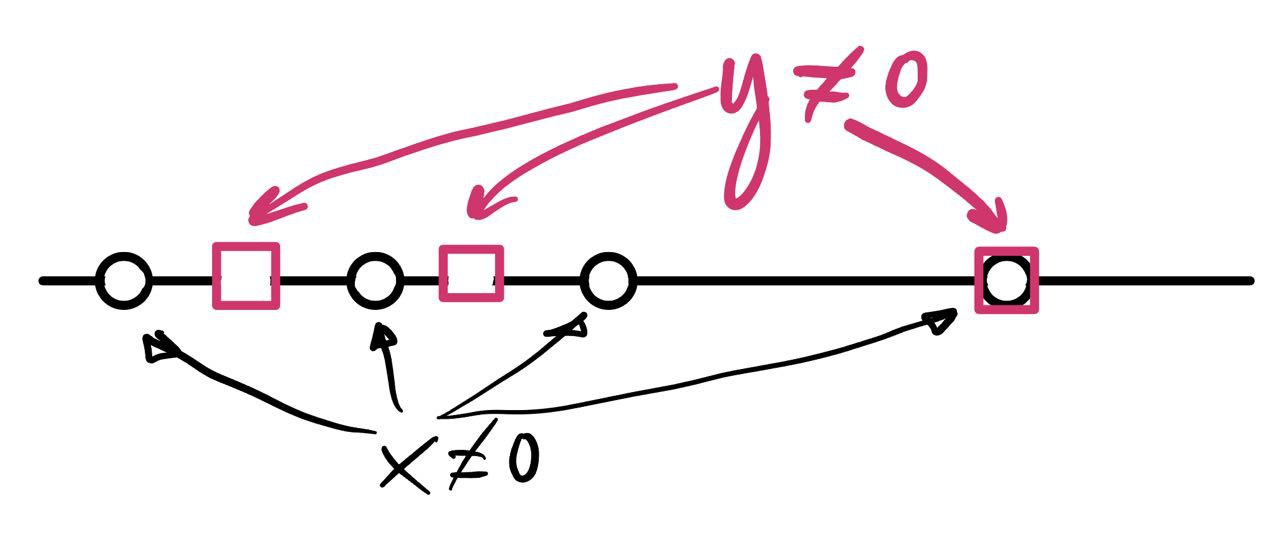
\includegraphics[width=0.4\textwidth]{123}
 	 	 	\end{center}
 	 	 \end{figure} \\
 	 	 
 	 	x+y может быть $\neq 0$ лишь на объединение множества, где $x \neq 0$ и $y \neq 0$ 
 	 	
 	 	Объединение конечных множеств кончено.\\
 	 	Замечание: если множество $I$ конечно, то $\oplus V_i = \prod_i$ (множества финитных функций)\\
 	 	
 	 	\subsection{Определение 5. Отображение из векторного пространства }
 	 	Отображение $\phi:  V \to W$ из векторного пространства $V$ в векторное пространство $V$ в векторное производство $V$ в векторное пространство $W$ называют линейным если $\forall x,y \ \in U \ \ \lambda, \mu \mathbb{R} \ \ \phi (\lambda y + \mu x) = \lambda \phi(x) + \mu \phi(y)$\\
 	 	Если $\phi: V \to V$, то $\phi$ называется линейным преобразованием или линейным оператором
\end{document}
		